\documentclass[fleqn,10pt]{SelfArx} % Document font size and equations flushed left

\usepackage{float}
\usepackage{graphicx}
\usepackage{caption}
\graphicspath{{../figures/}}

\newcommand{\beginsupplement}{%
        \setcounter{table}{0}
        \renewcommand{\thetable}{S\arabic{table}}%
        \setcounter{figure}{0}
        \renewcommand{\thefigure}{S\arabic{figure}}%
     }

\definecolor{color1}{RGB}{0,0,90} % Color of the article title and sections
\definecolor{color2}{RGB}{0,20,20} % Color of the boxes behind the abstract and headings

\JournalInfo{Supplementary Text} % Journal information ``Journal, Vol. XXI, No. 1, 1-5, 2015''
\Archive{ } % Additional notes (e.g. copyright, DOI, review/research article)

\PaperTitle{Supplementary results for: A meta-analysis of computational biology benchmarks reveals publication bias affects on speed and accuracy} % Article title

\Authors{Paul P. Gardner\textsuperscript{1,2}*, James Paterson\textsuperscript{1,2}, Fatemeh Ashari Ghomi\textsuperscript{1,2}, Sinan Uğur Umu\textsuperscript{1,2}, Stephanie McGimpsey\textsuperscript{1,2}} % Authors
\affiliation{\textsuperscript{1}\textit{School of Biological Sciences, University of Canterbury, Christchurch, New Zealand.}} % Author affiliation
\affiliation{\textsuperscript{2}\textit{Biomolecular Interaction Centre and the Bio-Protection Research Centre, University of Canterbury, Christchurch, New Zealand.}}
\affiliation{*\textbf{Corresponding author}: paul.gardner@canterbury.ac.nz} % Corresponding author

\Keywords{computational biology --- accuracy --- benchmarks --- meta-analysis --- software development} % Keywords - if you don't want any simply remove all the text between the curly brackets
\newcommand{\keywordname}{Keywords} % Defines the keywords heading name

%----------------------------------------------------------------------------------------
%	ABSTRACT
%----------------------------------------------------------------------------------------

\Abstract{In the below we provide additional results for our investigation of computational biology benchmarks.}

\begin{document}

\flushbottom % Makes all text pages the same height
\maketitle % Print the title and abstract box
%\tableofcontents % Print the contents section

\thispagestyle{empty} % Removes page numbering from the first page

%----------------------------------------------------------------------------------------
%	ARTICLE CONTENTS
%----------------------------------------------------------------------------------------

\onecolumn
\beginsupplement

\section*{Literature mining} % The \section*{} command stops section numbering


\begin{figure}[H]
\centering
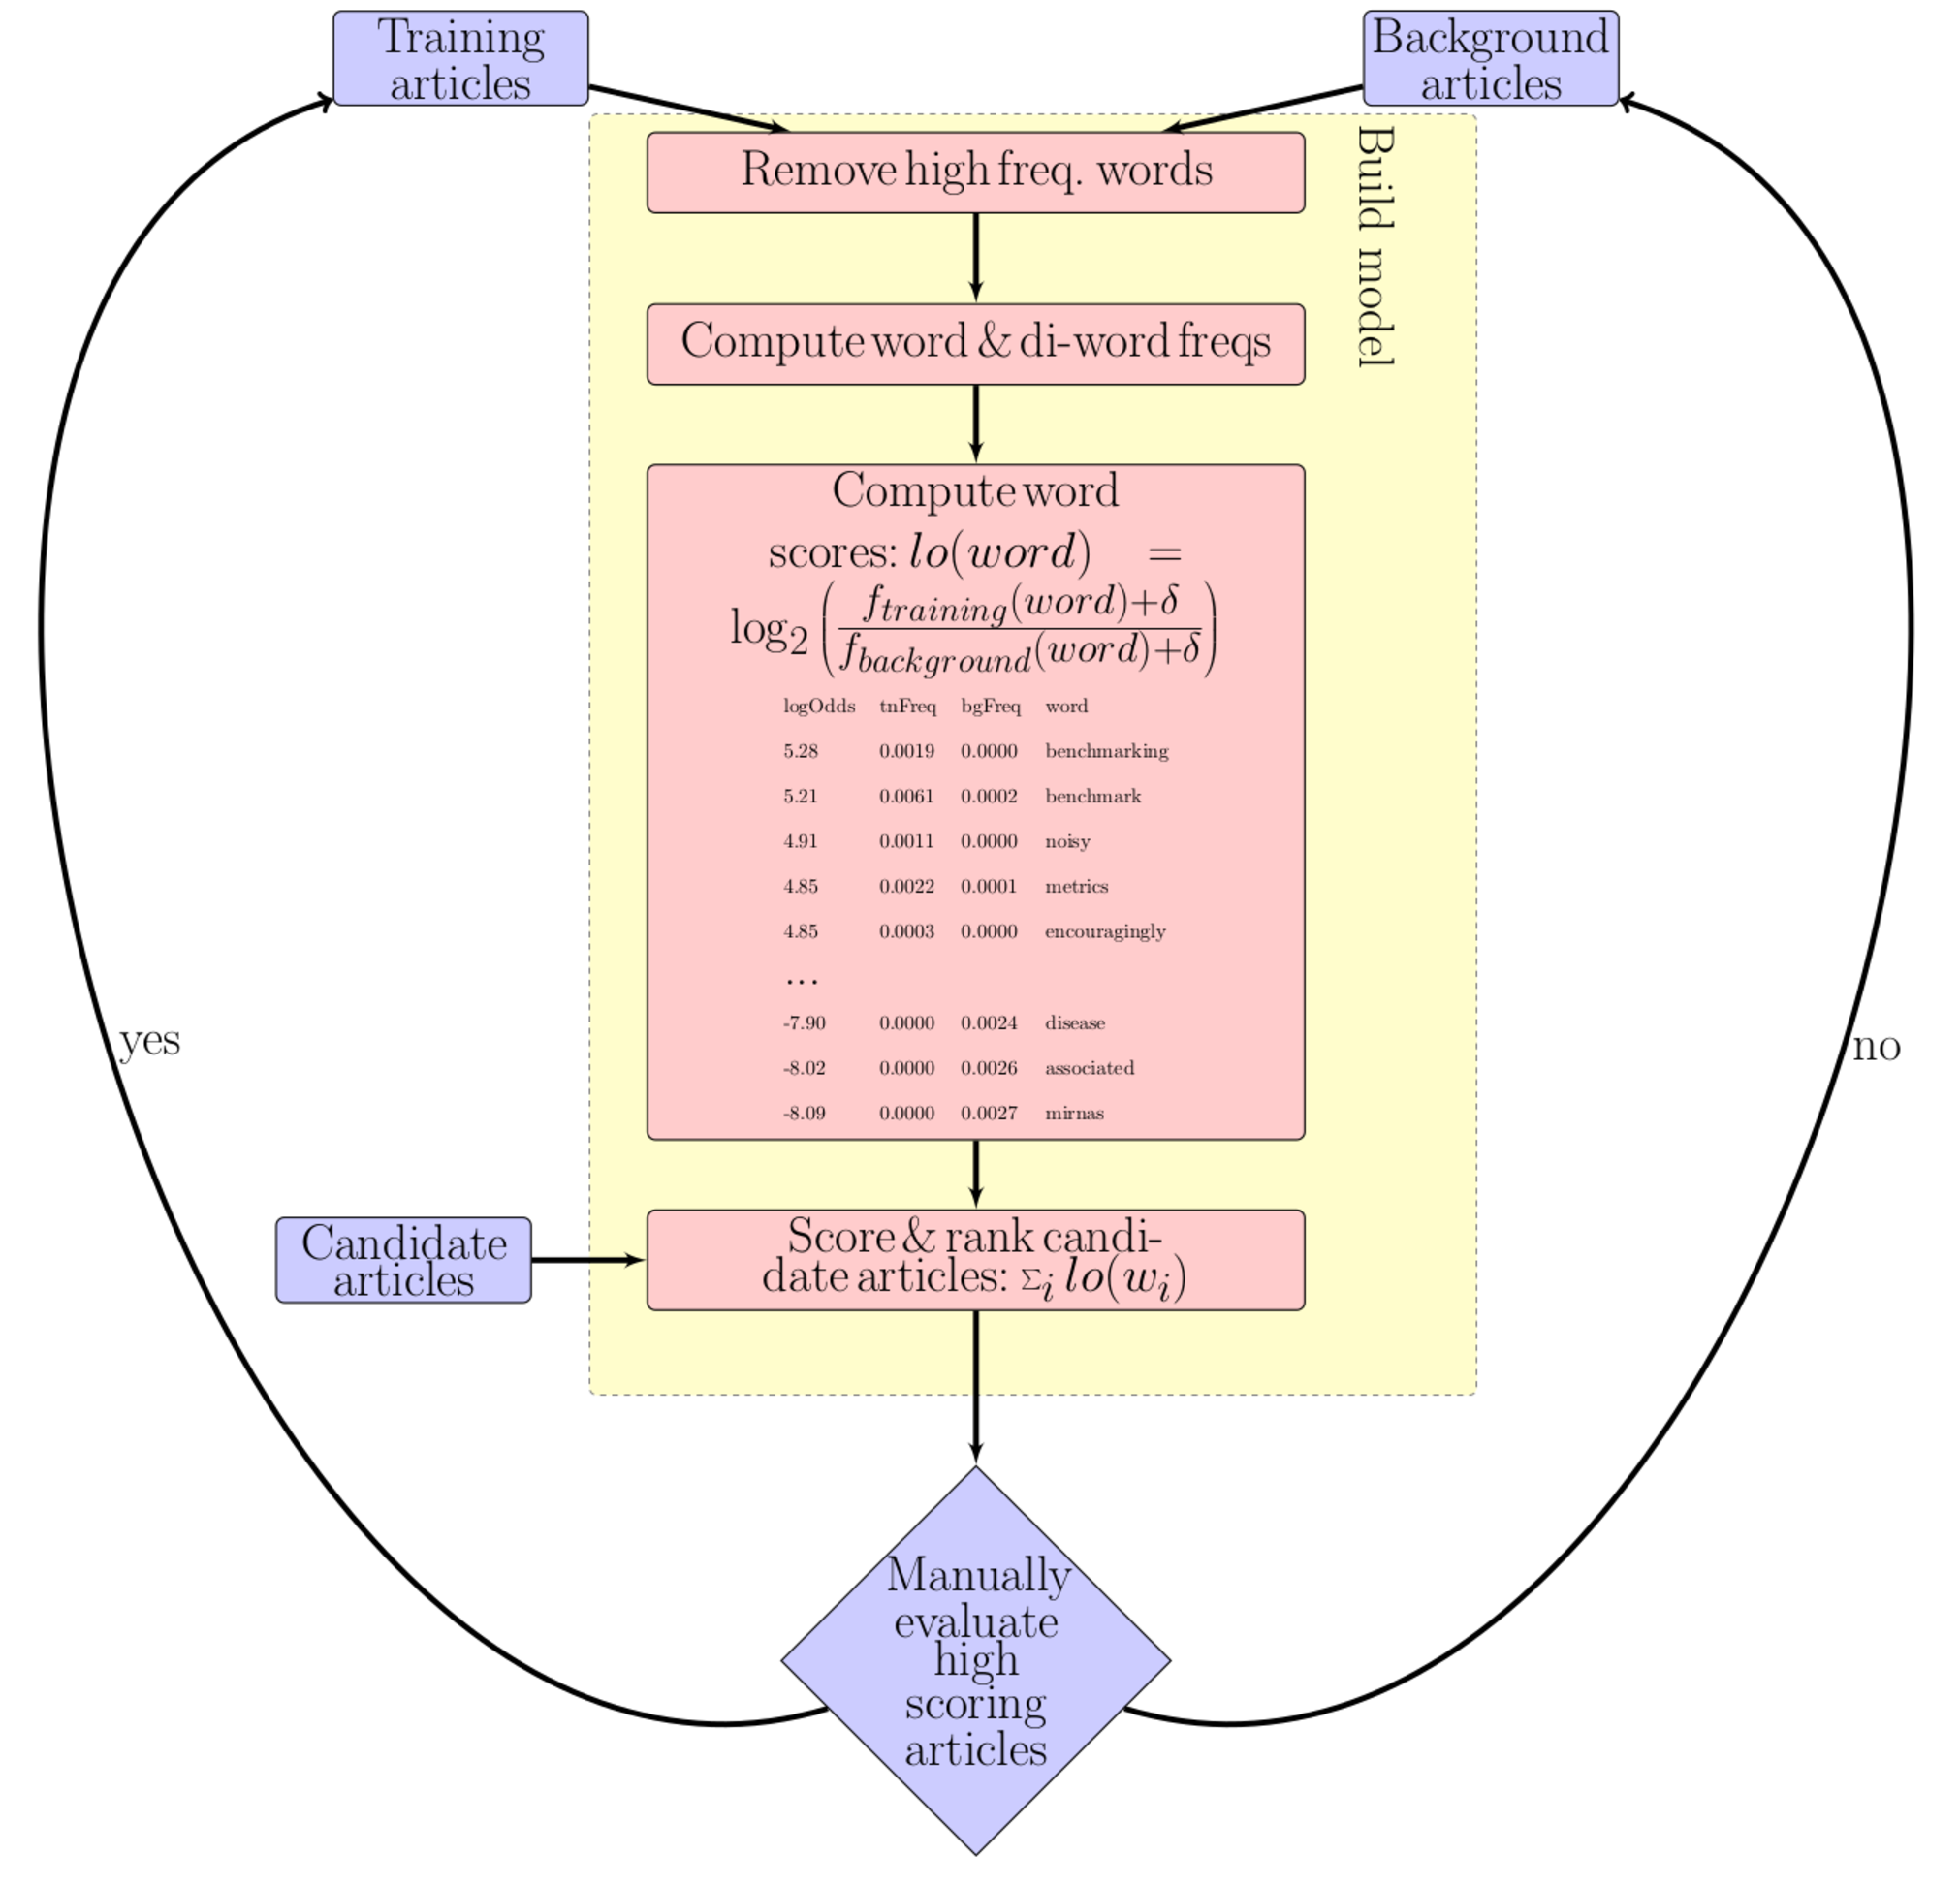
\includegraphics[height=0.7\textheight]{litMiningFlowDiagram-edited.pdf}
\caption{In order to improve the identification of benchmark articles
  that rank both accuracy and speed we developed a tool for ranking
  PubMed articles based upon word association scores (measured in
  ‘bits’). In brief, keywords were extracted from titles and abstracts
  for both training (in this case benchmark articles) and background
  articles (articles published between 2013 and 2015 with
  “bioinformatics” in the title or abstract). Log-odds ratios were
  computed for each keyword (measured in ‘bits’). Candidate articles
  that matched a hand-selected list of keywords associated with
  benchmarks were then scored and ranked with a “sum of bits”
  score. High ranking articles were then inspected, those that met our
  criteria were added to the training set, those that didn’t were
  added to the background set of articles.}
\label{fig:flow}
\end{figure}



\begin{figure}[H] \centering
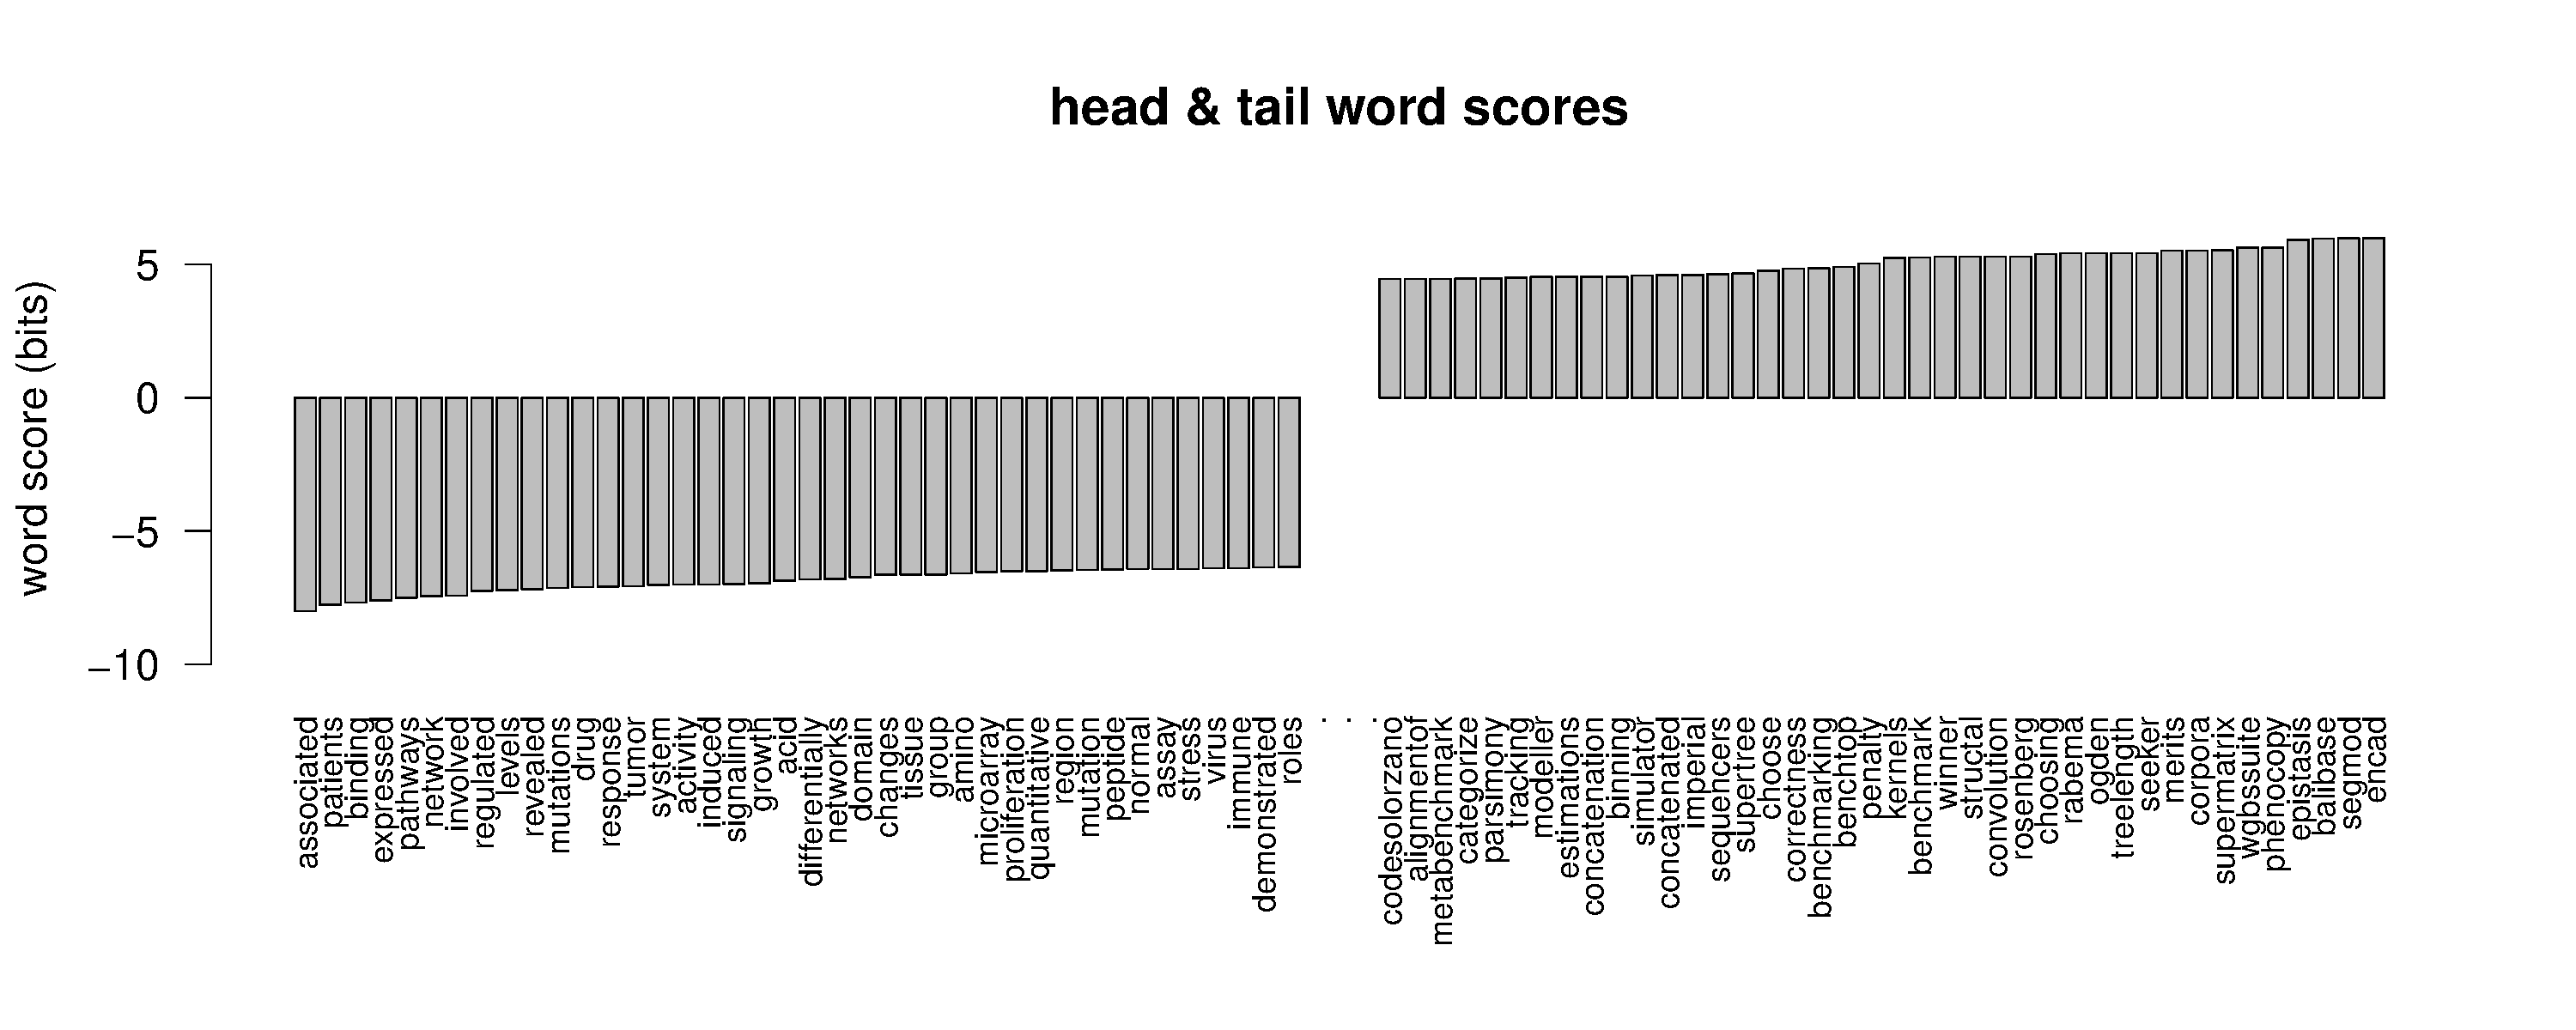
\includegraphics[width=1.05\textwidth]{wordScores.pdf} \caption{The 40
  highest and lowest scoring words that are associated with
  bioinformatic benchmark articles from the training benchmark articles,
  compared to the background articles. The log-odds ratios (measured
  in bits) are indicated on the y-axis. }
\label{fig:wordScores} \end{figure}


%% \clearpage
%% \newpage

%% \section*{R code ...}

%% {\tiny
%% \begin{verbatim}

%% \end{verbatim}
%% }


\clearpage
\newpage

\section*{Data mining} % The \section*{} command stops section numbering

\begin{figure}[H]
\centering
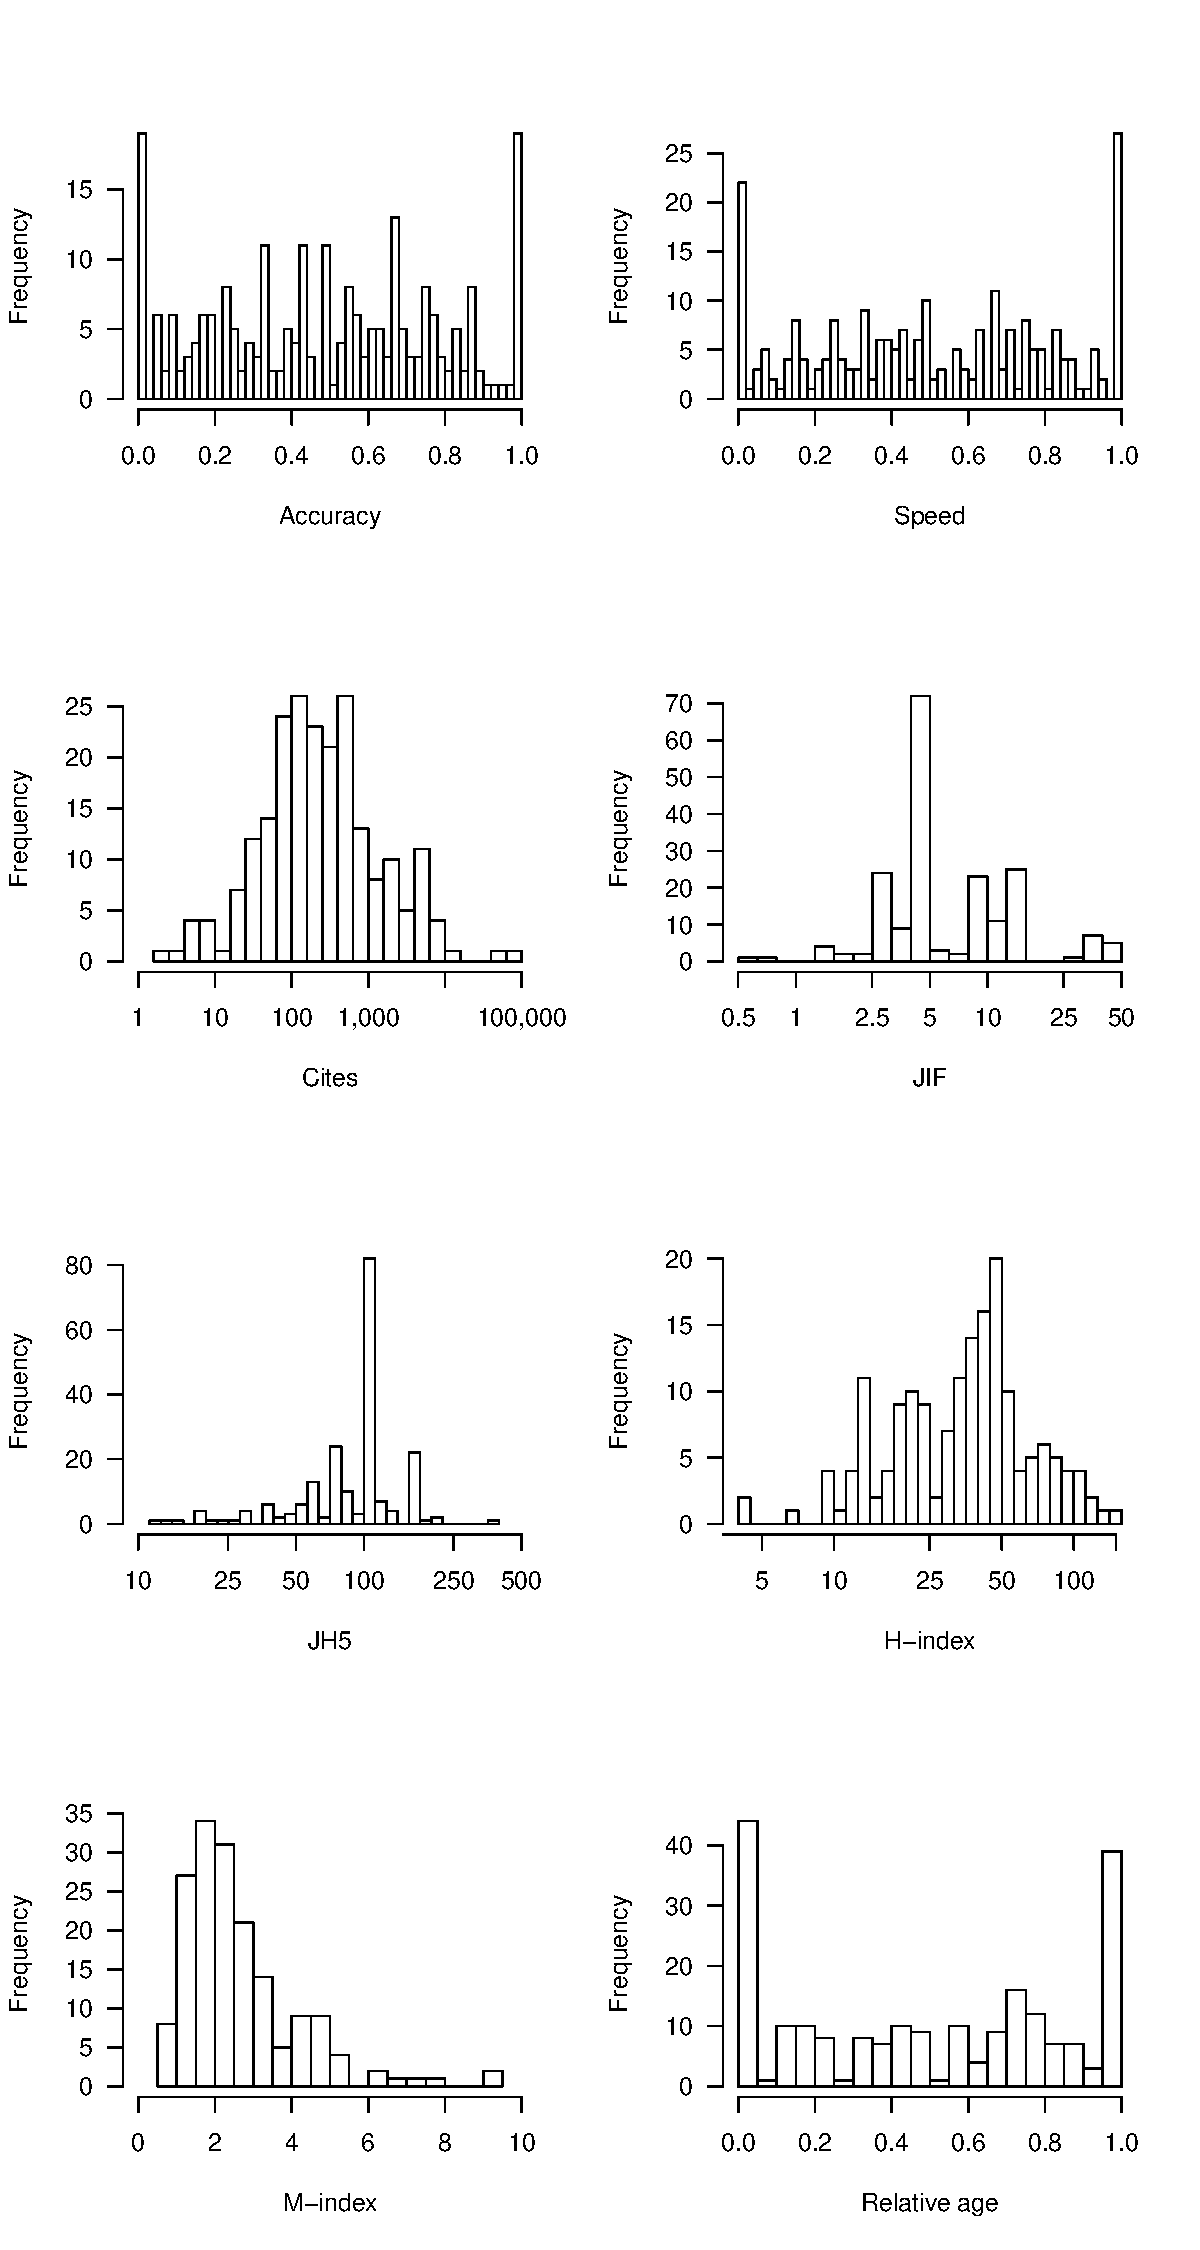
\includegraphics[width=0.75\textwidth]{supplementary-figures-small.pdf}
\caption{The distributions for the measures we expected to be
  predictive of software quality used in this study. These
are, reading from left to right, top to bottom: Accuracy -- the mean
normalised accuracy rank for each benchmarked method; Speed -- the
mean normalised speed rank for each benchmarked method; Cites -- the number of
citations to the most cited manuscript describing a method, data from GoogleScholar;
JIF -- the Journal Impact Factor to the highest impact journal that has published
a manuscript describing a method, data from 2014 Thompson-Reuters Citation Reports;
JH5 -- the Journal H5 index to the highest impact journal that has published
a manuscript describing a method, data from GoogleScholar 2015 Metrics;
H-index -- the H-index for the highest profile corresponding author from the
manuscripts describing a method, data from GoogleScholar User Profiles;
M-index -- the M-index (H-index/(\#years since first publication)) for the
highest profile corresponding author from the manuscripts describing a method,
data from GoogleScholar User Profiles;}
\label{fig:metricDistributions}
\end{figure}

\begin{figure}[H]
\centering
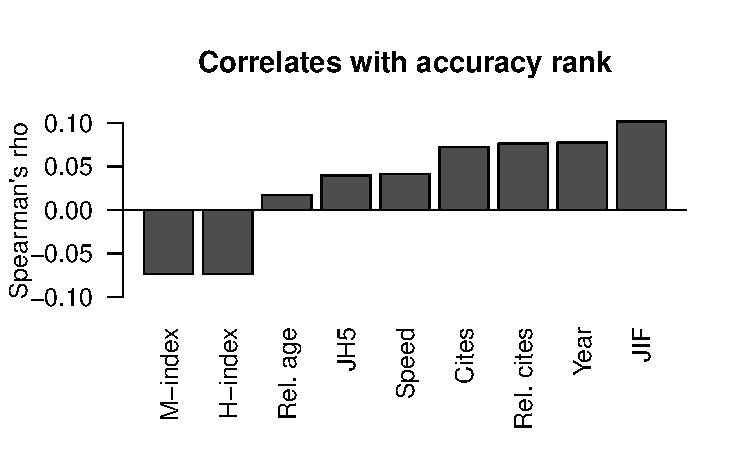
\includegraphics[width=0.45\textwidth]{spearmanBarplot.pdf}
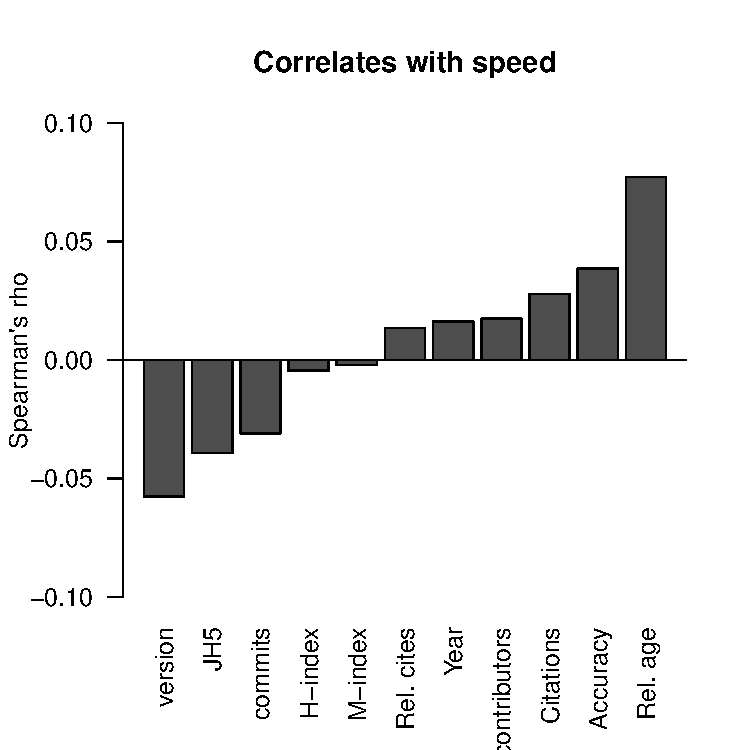
\includegraphics[width=0.45\textwidth]{spearmanBarplotSpeed.pdf}
\caption{The correlation between method accuracy (on the left) and
  method speed (on the right) and measures we expected to be
  predictive of software quality. E.g. author reputation measures
  (H-index, M-index), journal reputation (JH5 and JIF), number of
  users (citations and relative citations) or the recency of methods
  (year and relative age).  The correlations were estimated using
  Spearman's $\rho$. The signficant relationships are indicated with a
  ``*''. }
\label{fig:S2}
\end{figure}


\begin{figure}[H]
\centering
\includegraphics[width=0.5\textwidth]{smoothScatter-speed-vs-accuracy.pdf}
\caption{A smoothed color density representation of a scatterplot of
  normalised speed ranks and normalised accuracy ranks. Dark red
  regions are indicative of of a high density of points, blue shades
  indicate the reverse. The expected inverse relationship between
  speed and accuracy is indicated with a dashed black line, points
  above this line could be considered comparatively fast and accurate,
  points below are the reverse. A locally weighted regression (lowess)
  curve is shown in red.}
\label{fig:smoothScatterAccSpeed}
\end{figure}

\begin{figure}[H]
\centering
\includegraphics[width=0.85\textwidth]{smoothScatters.pdf}
\caption{A smoothed color density representation of a scatterplot of
  journal impact factors (JIF) on the left and number of citations on
  the right vs normalised accuracy ranks. As above, dark red regions
  are indicative of of a high density of points, blue shades indicate
  the reverse. The JIF for journals that are major publishers of
  bioinformatic software are indicated on the left. }
\label{fig:smoothScatters}
\end{figure}



\begin{figure}[H]
\centering
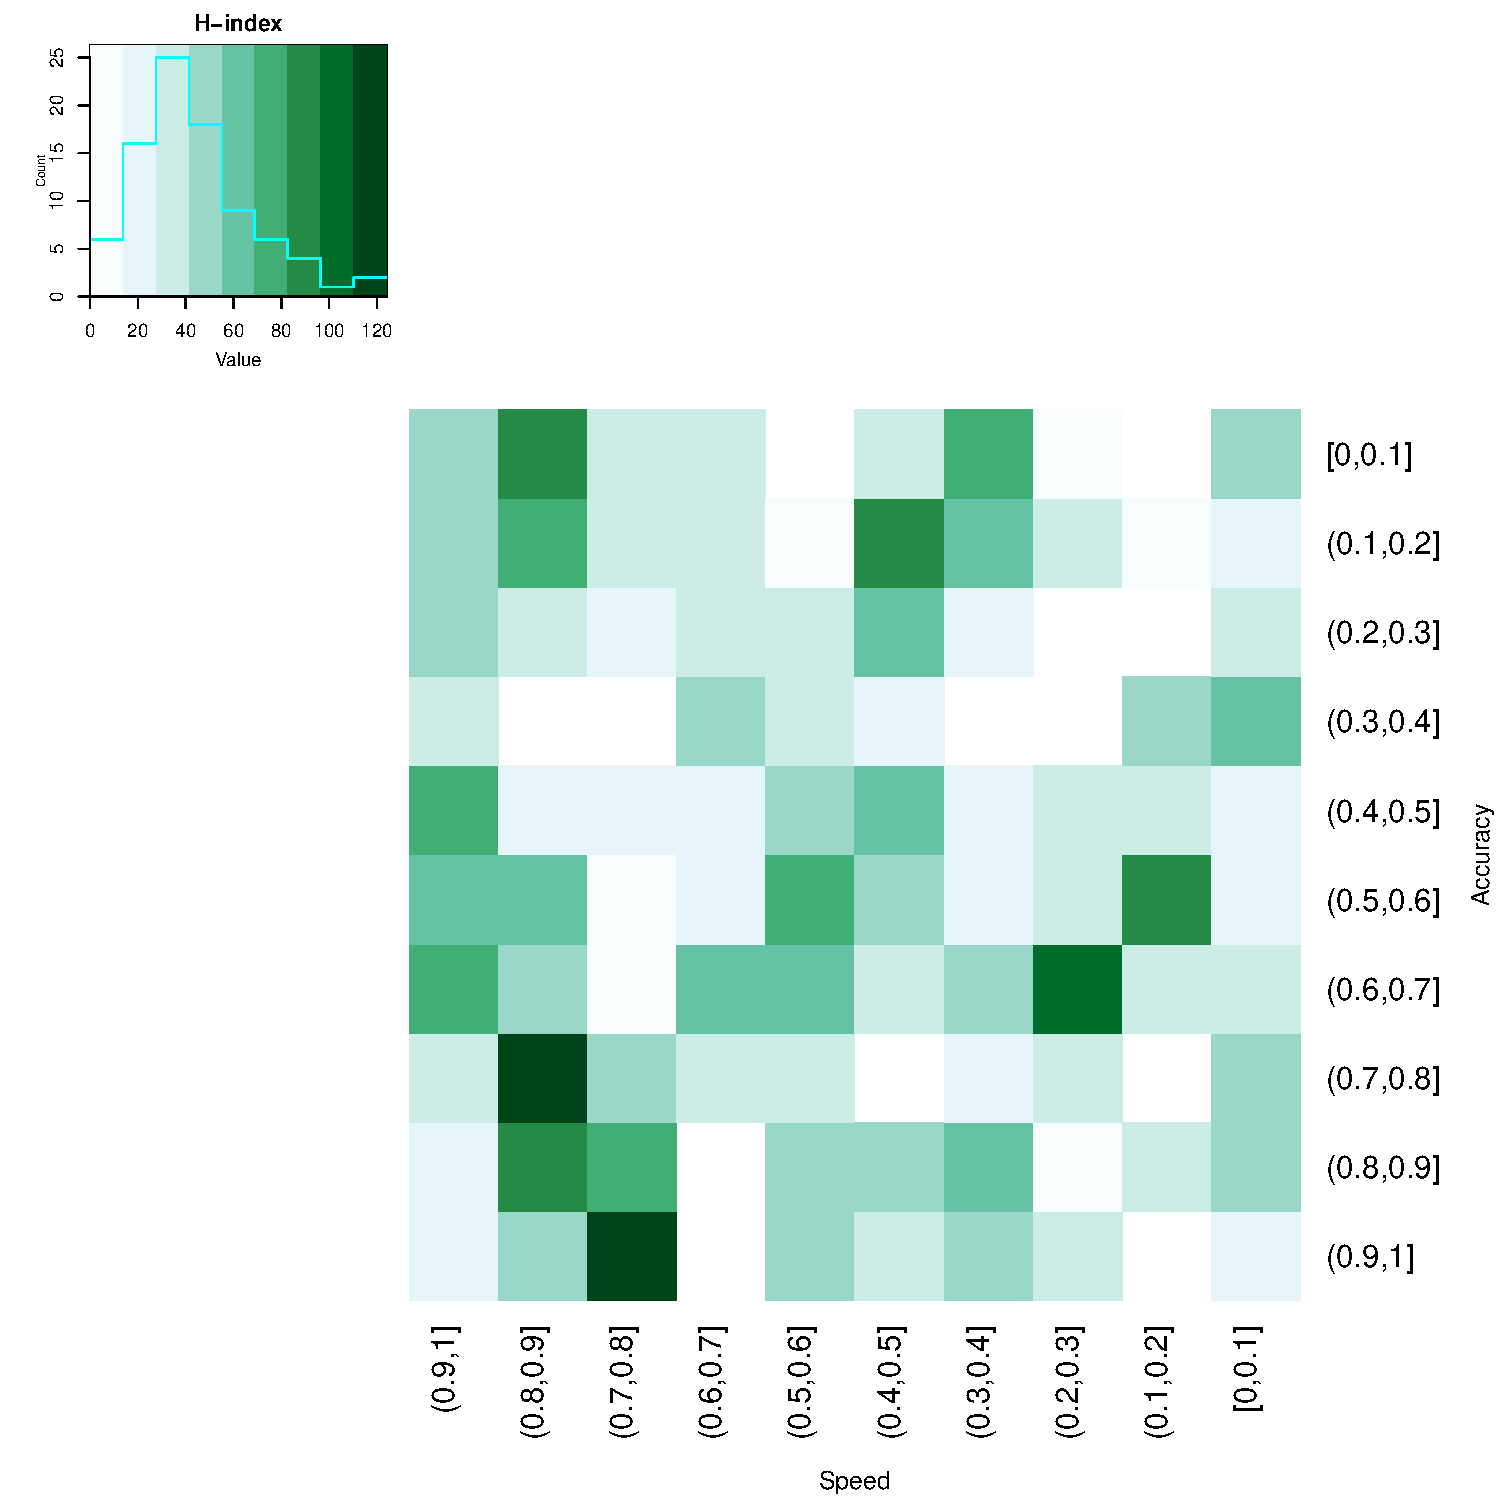
\includegraphics[width=0.45\textwidth]{hindex-SpeedVsAccuracy-heatmap.pdf}
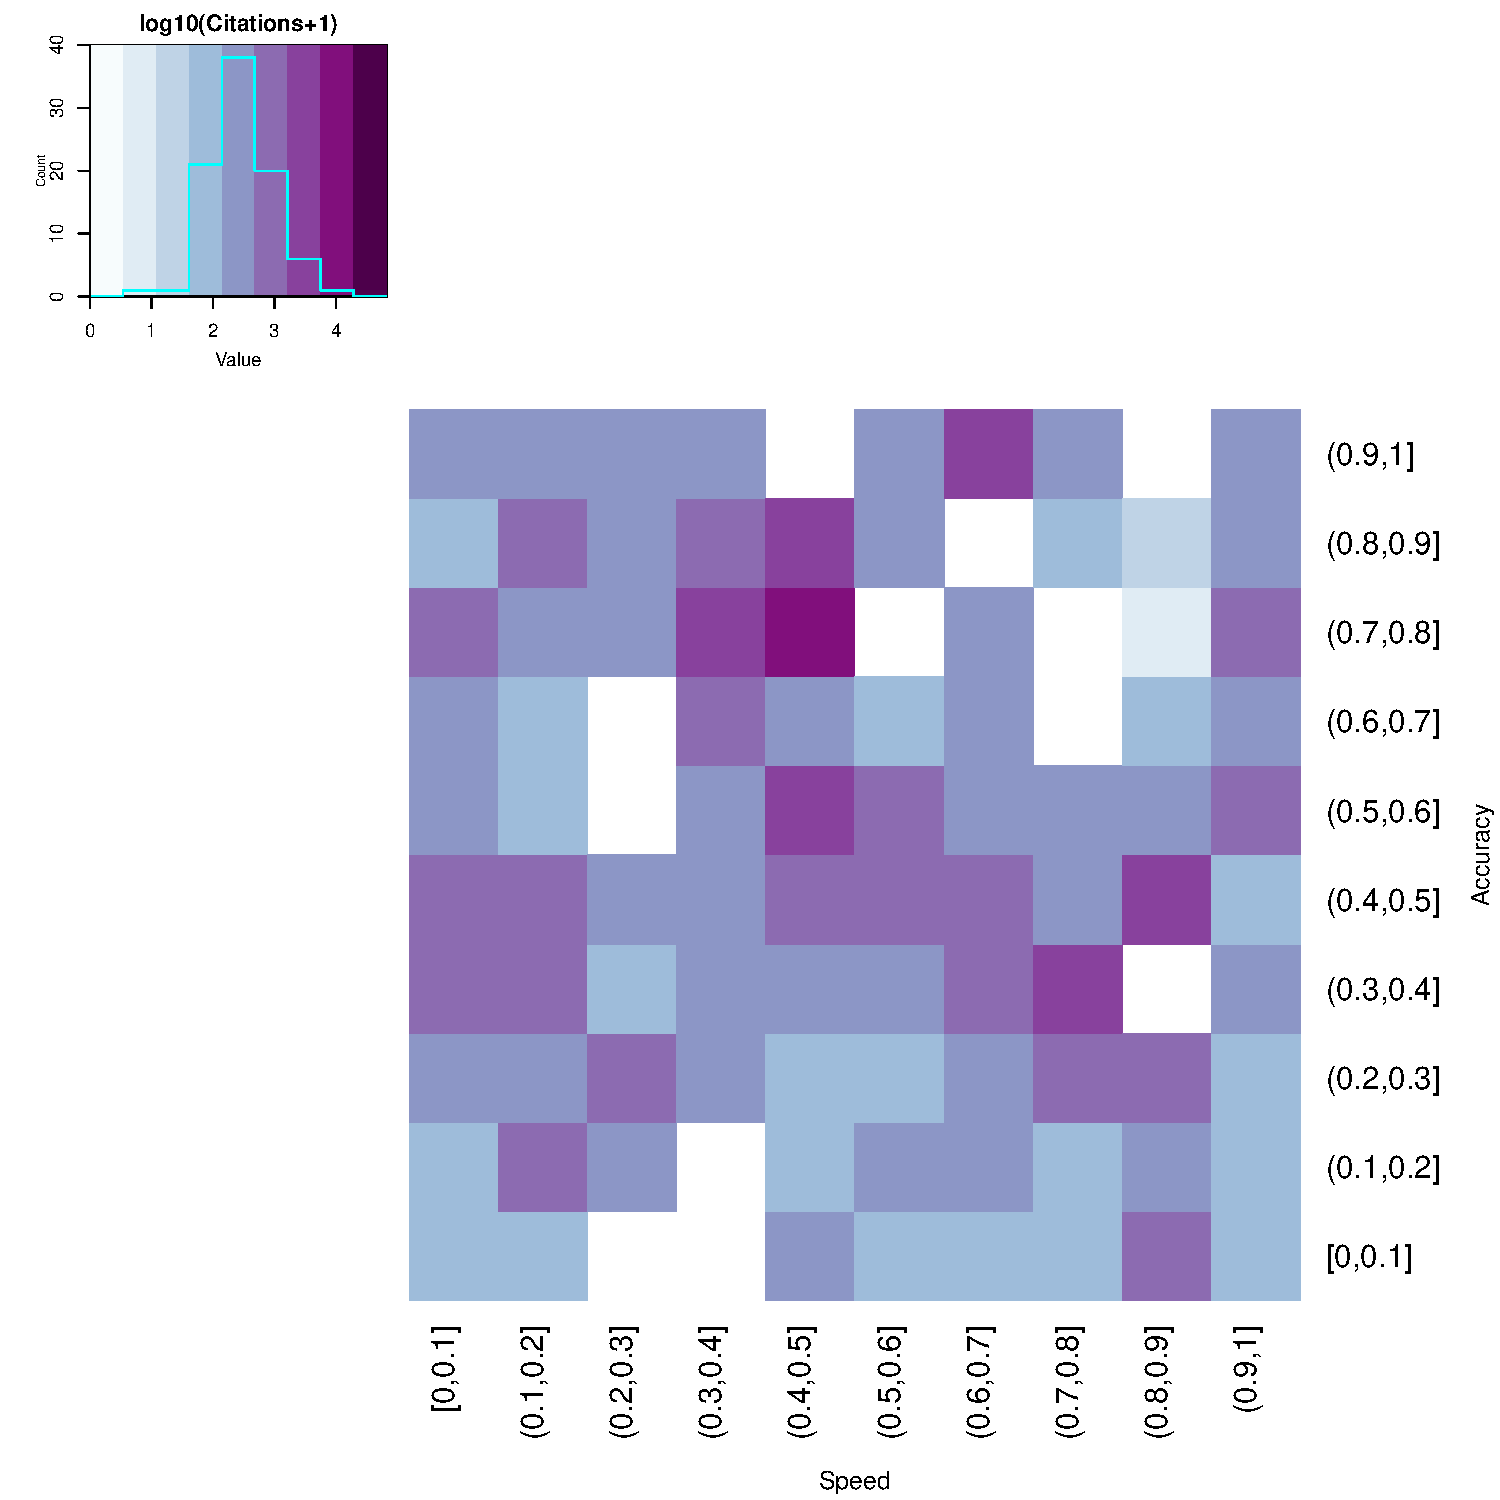
\includegraphics[width=0.45\textwidth]{cites-SpeedVsAccuracy-heatmap.pdf}
\caption{Heatmaps of normalised speed ranks and normalised accuracy
  ranks, both $x$ and $y$ dimensions are discretised into a $10 \times
  10$ matrix. The shading indicates median H-indices for corresponding
  authors (darker shade indicates a higher H) in the figure on the
  left. The shading indicates median citations (on a log scale), for
  software tools in the figure on the right. }
\label{fig:heatmaps}
\end{figure}


\begin{figure}[H]
\centering
\includegraphics[width=0.95\textwidth]{relAge-SpeedVsAccuracy-heatmap-edited.pdf}
\caption{{\bf A.} Violin plots for the relative age distribution for software tools in each of the 5 2x2 cells indicated in B. The five boxes correspond to the four extreme corners of the speed vs accuracy spectrum (i.e. slow and inaccurate, slow and accurate, fast and inaccurate, fast and accurate) and the central box (medium speed and medium accuracy). {\bf B.} A heatmap indicating the relative age of software in a range of relative accuracy and speed rankings. Blue colours indicate an abundance of older software tools in an accuracy and speed category, while light colours indicate younger software in an accuracy and speed category. }
\label{fig:ageplot}
\end{figure}


%----------------------------------------------------------------------------------------
%	REFERENCE LIST
%----------------------------------------------------------------------------------------
\bibliographystyle{unsrt}
\bibliography{paulall}

\end{document}








